\documentclass[tikz,border=6pt]{standalone}
\usepackage{pgfplots}
\pgfplotsset{compat=1.18}
\usepgfplotslibrary{colormaps}
\usetikzlibrary{arrows, arrows.meta, calc}
\usetikzlibrary{decorations.markings}


\usepackage{amssymb,amsmath,mathtools}

\usepackage[T1]{fontenc}
\usepackage[utf8]{inputenc}
\usepackage{newpxtext,newpxmath}
\usepackage{sectsty}

\newcommand{\Arg}{\textrm{Arg}}

\renewcommand{\Re}{\operatorname{\mathrm{Re}}}
\renewcommand{\Im}{\operatorname{\mathrm{Im}}}

\begin{document}
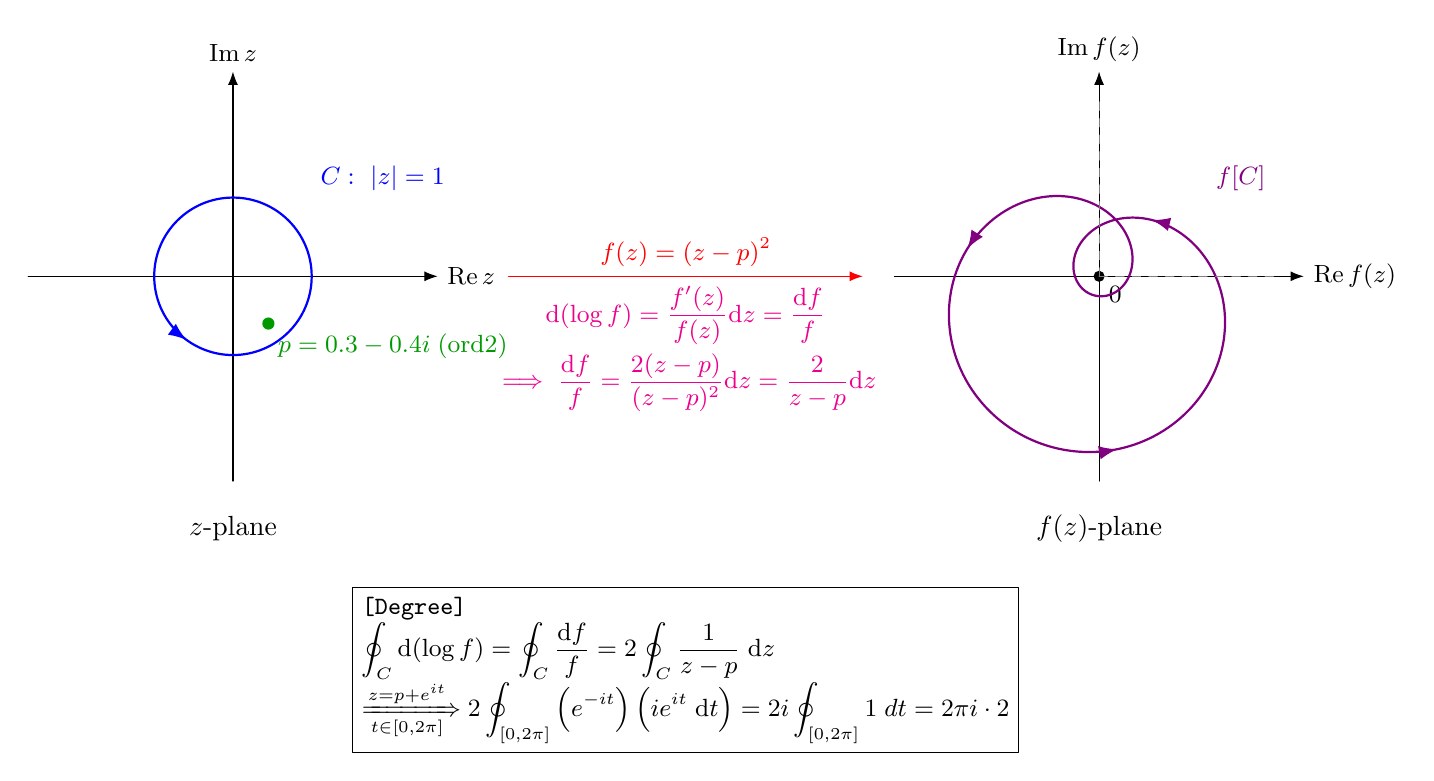
\begin{tikzpicture}[>=Latex, line cap=round, line join=round, font=\small]
%========================
% Left: z-plane
%========================
\begin{scope}[shift={(0,0)}]
	\node[font=\normalsize] at (0,-3.2) {$z$-plane};
	% axes
	\draw[->] (-2.6,0)--(2.6,0) node[right] {$\Re z$};
	\draw[->] (0,-2.6)--(0,2.6) node[above] {$\Im z$};
	
	% unit circle C (positively oriented) -- radius 1.5 for visibility
	\draw[blue,thick,postaction={decorate},
	decoration={markings, mark=at position 0.65 with {\arrow{>}}}]
	(0,0) circle (1);
	\node[blue] at (1.9,1.25) {$C:\ |z|=1$};
	
	% zero at p (order 2), choose concrete p inside C
	\fill[green!60!black] (0.45,-0.6) circle(2.2pt) node[below right] {$p=0.3-0.4i\; (\textrm{ord} 2)$};
%	\node[green!60!black] at (-1.8,1.7) {zero of order $2$};
%	\node[red] at (-1.8,-1.7) {poles: none};
\end{scope}

% function label + order via winding form
% annotation: coefficients from Cauchy integral formula at z_0=p
\draw[->, red] (3.5,0) -- (8,0) node[midway, above, align=center] {$\displaystyle
	f(z)=(z-p)^2$};
\draw[->, magenta, opacity=0] (3.5,0) -- (8,0) node[midway, below, align=center, opacity=1] {
	$\displaystyle\mathrm{d}(\log f)=\frac{f'(z)}{f(z)}\mathrm{d}z=\frac{\mathrm{d}f}{f}$\\ [2pt]
	$\displaystyle\implies\frac{\mathrm{d}f}{f}=\frac{2(z-p)}{(z-p)^2}\mathrm{d}z=\frac{2}{z-p}\mathrm{d}z$};

\node[draw=black, align=left] at (5.75,-5) {
	\texttt{[Degree]}\\
	$\displaystyle
	\oint_C \mathrm{d}(\log f)=\oint_C \frac{\mathrm{d}f}{f}=2\oint_C \frac{1}{z-p}\; \mathrm{d}z$ \\
	$\displaystyle\xRightarrow[{t\in[0,2\pi]}]{z=p+e^{it}}2\oint_{[0,2\pi]}\left(e^{-it}\right)\left(ie^{it}\; \mathrm{d}t\right)=2i\oint_{[0,2\pi]}1\; dt=2\pi i\cdot 2$
%	\\ [10pt]
%	\texttt{[Coefficient]}\\
%	$\displaystyle
%	a_0=f(p)=\frac{1}{2\pi i}\!\oint_C \frac{f(\zeta)}{\zeta-p}\,d\zeta=0$\\
%	$\displaystyle a_1=f'(p)=\frac{1}{2\pi i}\!\oint_C \frac{f(\zeta)}{(\zeta-p)^{2}}\,d\zeta=0,$\\[2pt]
%	$\displaystyle
%	a_2=\frac{f''(p)}{2!}
%	=\frac{1}{2\pi i}\!\oint_C \frac{f(\zeta)}{(\zeta-p)^{3}}\,d\zeta
%	=\frac{1}{2\pi i}\!\oint_C \frac{1}{\zeta-p}\,d\zeta=1.$
	};


%\draw[->] (3.5,0) -- (8,0) node[midway, above, align=center] {$\displaystyle
%	f(z)=(z-p)^{2}$};
%\draw[->, opacity=0] (3.5,0) -- (8,0) node[midway, below, align=center, opacity=1] {
%	$\displaystyle\oint_C \frac{df}{f}
%	=\oint_C \frac{2\,dz}{\,z-p\,}=2\pi i\cdot 2$\\
%	$\displaystyle
%	a_0=f(p)=\frac{1}{2\pi i}\!\oint_C \frac{f(\zeta)}{\zeta-p}\,d\zeta=0$\\
%	$a_1=f'(p)=\frac{1}{2\pi i}\!\oint_C \frac{f(\zeta)}{(\zeta-p)^{2}}\,d\zeta=0,$\\[2pt]
%	$\displaystyle
%	a_2=\frac{f''(p)}{2!}
%	=\frac{1}{2\pi i}\!\oint_C \frac{f(\zeta)}{(\zeta-p)^{3}}\,d\zeta
%	=\frac{1}{2\pi i}\!\oint_C \frac{1}{\zeta-p}\,d\zeta=1.$\\[4pt]
%	$\mathrm{wind}\big(f(C),0\big)=2
%	\ \Rightarrow\
%	\displaystyle \oint_C \frac{f'(z)}{f(z)}\,dz=2\pi i\cdot 2.$};

%========================
% Right: f(z)-plane
%========================
\begin{scope}[shift={(11,0)}]
	\node[font=\normalsize] at (0,-3.2) {$f(z)$-plane};
	% axes
	\draw[->] (-2.6,0)--(2.6,0) node[right] {$\Re f(z)$};
	\draw[->] (0,-2.6)--(0,2.6) node[above] {$\Im f(z)$};
	
	% origin
	\fill (0,0) circle(2pt) node[below right] {$0$};
	
	% image curve f(C): z = 1.5 e^{it} -> w = (z-p)^2
	% Let u = 1.5 cos t - 0.3, v = 1.5 sin t + 0.4.
	% Then w = (u + i v)^2 = (u^2 - v^2) + i (2 u v).
	\draw[violet,thick,
	postaction={decorate},
	decoration={markings,
			mark=at position 0.18 with {\arrow{>}},
			mark=at position 0.48 with {\arrow{>}},
			mark=at position 0.78 with {\arrow{>}}}]
	plot[domain=0:6.283, samples=600]
	({ (1*cos(\x r)-0.3)^2 - (1*sin(\x r)+0.4)^2 },
	{ 2*(1*cos(\x r)-0.3)*(1*sin(\x r)+0.4) });
	\node[violet] at (1.8,1.25) {$f[C]$};
	
	% dashed rays to visualize winding
	\draw[gray,dashed] (0,0) -- (2.3,0);
	\draw[gray,dashed] (0,0) -- (0,2.3);
\end{scope}
\end{tikzpicture}		
\end{document}